\chapter{一阶微分方程}
形如
\[
F(x,y,y')=0
\]
的微分方程被称为一阶微分方程. 由于并非所有一阶微分方程都有解，本章主要
介绍一些可解的方程以及相应的求法.

\section{线性方程}\label{sec:2.1}
\subsection{线性方程}
一阶线性微分方程
\[
y'+p(x)y=g(x)
\]
算是最为简单的一类微分方程了. 上一章中我们已经知道，若 $p(x),q(x)$ 连续，
则该方程在 $\R$ 上存在唯一解. 下面我们讨论该方程的解长什么样.

首先给出线性齐次方程的通解表达式.
\begin{thm}\label{thm:2.1.1}
一阶线性齐次微分方程
\begin{equation}\label{equ:2.1}
y'+p(x)y=0
\end{equation}
的通解表达式为
\begin{equation}\label{equ:2.2}
y=C\exp\left(-\int p(x)dx\right),
\end{equation}
其中 $C$ 为常数.
\begin{pf1}
对方程 (\ref{equ:2.1}) 两边同时乘以函数 $\exp\left(\int p(x)dx\right)$ 可得
\[
\left(y\exp\left(\int p(x)dx\right)\right)'=0,
\]
即
\[
y\exp\left(\int p(x)dx\right)=C,
\]
整理一下即可得到式 (\ref{equ:2.2}) 的通解.
\end{pf1}

基于定理 \ref{thm:2.1.1} 的思路和结果，我们对于非齐次方程的求解方法有两种途径.
\begin{thm}
一阶线性非齐次微分方程
\begin{equation}\label{equ:2.3}
y'+p(x)y=g(x)
\end{equation}
的通解表达式为
\begin{equation}\label{equ:2.4}
y=\exp\left(-\int p(x)dx\right)\left(C+\int g(x)\exp\left(\int p(x)dx\right)dx\right)
\end{equation}
\end{thm}
\begin{pf1}
\textbf{(i)}积分因子法：

对方程 (\ref{equ:2.3}) 两边同时乘以 $\exp\left(\int p(x)dx\right)$ 可得
\[
\left(y\exp\left(\int p(x)dx\right)\right)'=g(x)\exp\left(\int p(x)dx\right),
\]
对上式两边积分，再整理即可得到式 (\ref{equ:2.4}).

\textbf{(ii)}常数便易法：

定理 \ref{thm:2.1.1} 中已经得到齐次方程的通解 (\ref{equ:2.2})，将其中的常数 $C$ 换成
待定函数 $C(x)$，即令
\begin{equation}\label{equ:2.5}
y=C(x)\exp\left(-\int p(x)dx\right).
\end{equation}
计算 $y$ 的导数
\[
y'=C'(x)\exp\left(-\int p(x)dx\right)-p(x)C(x)\exp\left(-\int p(x)dx\right).
\]
将 $y$ 和 $y'$ 代入 (\ref{equ:2.3}) 整理得到代求函数 $C(x)$ 满足
\[
C'(x)=g(x)\exp\left(\int p(x)dx\right),
\]
积分可得
\[
C(x)=C+\int g(x)\exp\left(\int p(x)dx\right)dx
\]
最后将 $C(x)$ 表达式代入 $(\ref{equ:2.5})$ 即可得到式 (\ref{equ:2.4}).
\end{pf1}
\end{thm}

\subsection{Bernoulli 方程}

线性方程的一个直接推广就是 Bernoulli 方程，它在实际中也经常出现.

\begin{deff}[(Bernoulli 方程)]
形如
\begin{equation}\label{equ:2.6}
y'+p(x)y=g(x)y^{\alpha}
\end{equation}
的一阶微分方程称为 \textbf{Bernoulli 方程}，其中 $\alpha\in\R$ 且 $\alpha\neq 0,1$.
\end{deff}

\begin{rmk}
当 $\alpha=0$ 时，方程 (\ref{equ:2.6}) 就是线性非齐次方程；当 $\alpha=1$ 时，方程
可分离变量，这两种情形我们已经讨论过了，因此 Bernoulli 方程专指 $\alpha\neq 0,1$
的情形.
\end{rmk}

Bernoulli 方程虽然不是线性方程，但可以通过一个简单的变量替换化为线性方程，
从而使用上一小节的方法求解.

\begin{thm}
Bernoulli 方程 (\ref{equ:2.6}) 经变量替换 $z=y^{1-\alpha}$ 后可化为关于 $z$ 的
一阶线性微分方程
\begin{equation}\label{equ:2.7}
z'+(1-\alpha)p(x)z=(1-\alpha)g(x).
\end{equation}
\end{thm}
\begin{pf1}
设 $z=y^{1-\alpha}$，则
\[
z'=(1-\alpha)y^{-\alpha}y'.
\]
将方程 (\ref{equ:2.6}) 两边同时乘以 $(1-\alpha)y^{-\alpha}$，得
\[
(1-\alpha)y^{-\alpha}y'+(1-\alpha)p(x)y^{1-\alpha}=(1-\alpha)q(x),
\]
即
\[
z'+(1-\alpha)p(x)z=(1-\alpha)q(x).
\]
这就是关于 $z$ 的一阶线性微分方程，其通解可由定理 \ref{thm:2.1.1} 后面的公式
(\ref{equ:2.4}) 直接写出：
\[
z=\exp\left(-\int (1-\alpha)p(x)dx\right)\left(C+\int (1-\alpha)q(x)\exp\left(\int (1-\alpha)p(x)dx\right)dx\right).
\]
整理一下指数上的符号并将 $z=y^{1-\alpha}$ 代回即可得到 Bernoulli 方程\ref{equ:2.6}的通解.
\end{pf1}

\begin{eg}
求解方程
\[
y'+\frac{1}{x}y=x^2y^3.
\]
\begin{pf2}
这是一个 $\alpha=3$ 的 Bernoulli 方程. 令 $z=y^{-2}$，则 $z'=-2y^{-3}y'$.
将原方程两边乘以 $-2y^{-3}$ 再代入 $z$，得
\[
z'-\frac{2}{x}z=-2x^2.
\]
这是关于 $z$ 的线性方程，解得
\[
z=-2x^3+Cx^2.
\]
将 $z=y^{-2}$ 代回，得到原方程的通解
\[
y^{-2}=-2x^3+Cx^2.
\]
另外，原方程还有解 $y=0$（分离变量时丢掉的常数解）.
\end{pf2}
\end{eg}

\begin{rmk}
在 Bernoulli 方程的求解过程中，将方程除以 $y^{\alpha}$ 时，
实际上默认了 $y\neq 0$. 因此 $y=0$ 可能是一个常数解，需要单独检验是否满足
原方程，如上面的例子所示.
\end{rmk}


\section{变量可分离的方程}\label{sec:2.2}
\subsection{变量可分离方程的求解}
形如
\begin{equation}\label{equ:2.8}
\frac{dy}{dx} = f(x)g(y)
\end{equation}
的方程称为 \textbf{变量可分离方程}. 下面给出这类方程的求解方法.

\begin{thm}
若 $g(y)\neq0$，则方程 (\ref{equ:2.8}) 的通解为
\begin{equation}\label{equ:2.9}
\int\frac{dy}{g(y)}=\int f(x)dx +c.
\end{equation}
\end{thm}
\begin{pf1}
方程等价于
\[
dy=f(x)g(y)dy,
\]
再把 $g(y)$ 移到等式左边，得到
\begin{equation}\label{equ:2.10}
\frac{dy}{g(y)}=f(x)dx.
\end{equation}
由于 $\int\frac{dy}{g(y)}$ 对 $y$ 求导会得到 $\frac{1}{g(y)}$, 
因此 $\frac{dy}{g(y)}=d\left(\int\frac{dy}{g(y)}\right)$. 等式右边
同理，因此上式等价于
\[
d\left(\int\frac{dy}{g(y)}\right)=d\left(\int f(x)dx\right),
\]
即
\[
\int\frac{dy}{g(y)}=\int f(x)dx+c.
\]
得到变量可分离方程的通解式 (\ref{equ:2.9}).
\end{pf1}
\begin{rmk}
\begin{description}
\item[(i)] 形式上，可以将微分方程 (\ref{equ:2.10}) 的等式两边积分直接得到
通解 (\ref{equ:2.9})，这是莱布尼茨符号的便利之处.
\item[(ii)] 实际上，若给定初始条件 $y(x_0)=y_0$, 式 (\ref{equ:2.10}) 等价于
$\int_{y_0}^{y}\frac{ds}{g(s)}=\int_{x_0}^{x}f(t)dt$，读者可自行给出严谨证明.
\item[(iii))] 当 $g(y)=0$ 是，需将其代入方程 \ref{equ:2.8} 进行单独检验. 由于
检验较为简单，后续我们不再单独说明.
\end{description}

\end{rmk}
\subsection{齐次方程}
形如
\begin{equation}\label{equ:2.11}
\frac{dy}{dx}=F(\frac{y}{x})
\end{equation}
的方程称为 \textbf{齐次方程}. 它可以通过引入新变量 $z=y/x$ 变成
变量可分离方程.

\begin{thm}
齐次方程 (\ref{equ:2.11}) 经变量替换 $z=y/x$ 后可化为变量可分离方程
\begin{equation}\label{equ:2.12}
\frac{dz}{dx}=\frac{F(z)-z}{x}.
\end{equation}
\end{thm}
\begin{pf1}
令 $z=y/x$，即 $y=xz$，两边对 $x$ 求导得
\[
\frac{dy}{dx}=z+x\frac{dz}{dx}.
\]
将其代入方程 (\ref{equ:2.11})，得
\[
z+x\frac{dz}{dx}=F(z),
\]
整理即得方程 (\ref{equ:2.12})，这是关于 $z$ 的变量可分离方程.
\end{pf1}

\begin{eg}
求解方程
\[
(y+\sqrt{x^2+y^2})dx=xdy.
\]
\begin{pf2}
当 $x\neq0$ 时, 原方程可写为
\[
\frac{dy}{dx}=\frac{y+\sqrt{x^2+y^2}}{x},
\]
这是齐次方程. 当 $x>0$ 时, 令 $z=y/x$，则原方程化为
\[
\frac{dz}{dx}=\frac{\sqrt{1+z^2}}{x}.
\]
分离变量得
\[
\frac{dz}{\sqrt{1+z^2}}=\frac{dx}{x},
\]
两边积分得
\[
\ln(z+\sqrt{1+z^2})=\ln x+c_1,
\]
整理得 $z+\sqrt{1+z^2}=cx$，其中 $c>0$. 将 $z=y/x$ 代回，得到原方程的通解
\[
y+\sqrt{x^2+y^2}=cx^2,\quad x>0.
\]
当 $x<0$ 时，$\dfrac{\sqrt{x^2+y^2}}{x}=-\sqrt{1+z^2}$，同理可得通解
\[
\sqrt{x^2+y^2}-y=c,\quad x<0.
\]
另外，$x=0$ 也是原方程的解.
\end{pf2}
\end{eg}

\begin{eg}
求解方程
\begin{equation}\label{equ:2.13}
\frac{dy}{dx}=f\left(\frac{a_1x+b_1y+c_1}{a_2x+b_2y+c_2}\right)
\end{equation}
\end{eg}
\begin{pf1}
考虑两条直线 $a_1 x+b_1 y+c_1=0$ 和 $a_2 x+b_2 y+c_2=0$，若
两条直线平行，则存在 k, 使得方程 (\ref{equ:2.13}) 等价于
\[
\frac{dy}{dx}=f(k),
\]
于是
\[
y=f(k)x+c.
\]

若两条直线相交于 $(x_0,y_0)$, 则可以通过变换坐标系使两条直线经过原点（齐次化），
即令 $m=x-x_0, n=y-y_0$，于是原方程 (\ref{equ:2.13}) 等价于
\[
\frac{dn}{dm}=f\left(\frac{a_1m+b_1n}{a_2m+b_2n}\right),
\]
再变为齐次方程
\[
\frac{dn}{dm}=f\left(\frac{a_1+b_1z}{a_2+b_2z}\right),\quad z=\frac{n}{m}
\]
即可求解.
\end{pf1}


\section{全微分方程}\label{sec:2.3}
\subsection{全微分方程}
若存在一个连续可微的二元函数 $u=F(x,y)$, 使得某微分方程形如
\[
F_xdx+F_ydy=0,
\]
则称该方程为全微分方程，其中 $F_x,F_y$ 分别表示 $F$ 对 $x,y$ 的偏导数. 显然该方程的解为 $F(x,y)=C$.

我们发现全微分方程的求解是简单的，因此若我们能确定哪些方程是全微分方程，理论上我们能
轻易求出该方程的通解. 下面给出判定全微分方程的充要条件.
\begin{thm}\label{thm:2.3.1}
设 $M(x,y),N(x,y)$ 在单连通区域 $D$ 内具有连续的一阶偏导数，则方程
\begin{equation}\label{equ:2.14}
M(x,y)dx+N(x,y)dy=0
\end{equation}
为全微分方程的充要条件是
\begin{equation}\label{equ:2.15}
M_y=N_x
\end{equation}
在 $D$ 内恒成立.
\end{thm}
\begin{pf1}
\textbf{(i)} 必要性. 若 (\ref{equ:2.14}) 是全微分方程，则存在 $F(x,y)$，使得
\[
dF=F_xdx+F_ydy=Mdx+Ndy,
\]
即
\[
M=F_x,\quad N=F_y.
\]
由于 $M,N$ 具有连续的一阶偏导数，故 $F$ 的二阶混合偏导数连续，于是
\[
M_y=F_{xy}=F_{yx}=N_x.
\]

\textbf{(ii)} 充分性. 设 (\ref{equ:2.15}) 在 $D$ 内恒成立. 任取 $(x_0,y_0)\in D$，对任意 $(x,y)\in D$，定义
\[
F(x,y)=\int_{(x_0,y_0)}^{(x,y)}Mdx+Ndy,
\]
其中积分沿 $D$ 内连接 $(x_0,y_0)$ 与 $(x,y)$ 的曲线进行. 首先说明该积分与路径无关. 设
$\Gamma_1,\Gamma_2$ 是 $D$ 内连接这两点的两条曲线，它们围成闭曲线 $\Gamma$，且 $\Gamma$ 所围区域
$D_\Gamma\subset D$，由 Green 公式得
\[
\oint_{\Gamma}Mdx+Ndy=\iint_{D_\Gamma}\left(N_x-M_y\right)dxdy=0,
\]
故 $F(x,y)$ 的定义是合理的.

再取从 $(x_0,y_0)$ 到 $(x,y)$ 的曲线，并沿从 $(x,y)$ 到 $(x+\Delta x,y)$ 的水平线段积分，
由积分与路径无关可得
\[
F(x+\Delta x,y)-F(x,y)=\int_{x}^{x+\Delta x}M(t,y)dt,
\]
于是
\[
F_x=M(x,y).
\]
同理可得
\[
F_y=N(x,y).
\]
因此
\[
dF=Mdx+Ndy,
\]
即方程 (\ref{equ:2.14}) 是全微分方程. 定理得证.
\end{pf1}

上面的证明利用线积分构造出 $F$. 除此之外，我们还经常用偏积分法和凑微分法求 $F$.下面用两个例子分别介绍这两种方法.

\begin{eg}
求解方程
\[
(2x+y)dx+(x+2y)dy=0.
\]
\begin{pf2}
这里 $M=2x+y$, $N=x+2y$，且
\[
M_y=1=N_x,
\]
故原方程是全微分方程. 所谓偏积分法，就是先由 $M=F_x$ 将 $M$ 关于 $x$ 积分，得
\[
F(x,y)=\int(2x+y)dx=x^2+xy+\varphi(y),
\]
其中 $\varphi(y)$ 是待定函数. 再利用 $F_y=N$ 得
\[
x+\varphi'(y)=x+2y,
\]
即 $\varphi'(y)=2y$，故 $\varphi(y)=y^2$. 于是
\[
F(x,y)=x^2+xy+y^2,
\]
原方程的通解为
\[
x^2+xy+y^2=C.
\]
\end{pf2}
\end{eg}

\begin{eg}
求解方程
\[
(y\cos x+2xe^y)dx+(\sin x+x^2e^y+2y)dy=0.
\]
\begin{pf2}
这里 $M=y\cos x+2xe^y$, $N=\sin x+x^2e^y+2y$，且
\[
M_y=\cos x+2xe^y=N_x,
\]
故原方程是全微分方程. 所谓凑微分法，就是把方程左端适当分组，使每一组恰好是某个函数的全微分：
\[
y\cos x dx+\sin x dy=d(y\sin x),
\]
\[
2xe^y dx+x^2e^y dy=d(x^2e^y),
\]
\[
2y dy=d(y^2),
\]
于是原方程可写为
\[
d(y\sin x+x^2e^y+y^2)=0,
\]
其通解为
\[
y\sin x+x^2e^y+y^2=C.
\]
\end{pf2}
\end{eg}
\begin{rmk}
一般来说，凑微分法的效率高于其它方法（包括 \ref{sec:2.1} 和 \ref{sec:2.2}），
因此在考场中建议先观察尝试凑微分.
\end{rmk}

\subsection{积分因子}
大部分时候 $Mdx+Ndy=0$ 不是全微分方程，这时候我们想到 \ref{sec:2.1}
中的积分因子法让它变成全微分方程，即寻找二元函数 $\mu(x,y)$ 使得
\[
\mu(x,y)M(x,y)dx+\mu(x,y)N(x,y)dy=0
\]
为全微分方程.

由定理 \ref{thm:2.3.1} 可知，$\mu$ 为积分因子当且仅当
\begin{equation}\label{equ:2.16}
(\mu M)_y=(\mu N)_x,
\end{equation}
展开即
\begin{equation}\label{equ:2.17}
N\mu_x-M\mu_y=\mu(M_y-N_x).
\end{equation}
一般说来，求解偏微分方程 (\ref{equ:2.17}) 并不比求解原方程容易. 于
是我们首先考虑 $\mu$ 只与一个变量有关，此时 (\ref{equ:2.17}) 会退
化为一个常微分方程，从而可以求出 $\mu$. 下面给出这一情形下的充要条件.

\begin{thm}\label{thm:2.3.2}
设 $M,N$ 在区域 $D$ 内具有连续的一阶偏导数.
\begin{description}
\item[(i)] 当 $N\neq0$ 时，方程 (\ref{equ:2.14}) 有仅依赖于 $x$ 的积分因子的充要条件是
\[
\frac{1}{N}(M_y-N_x)
\]
仅依赖于 $x$. 此时积分因子为
\begin{equation}\label{equ:2.18}
\mu(x)=\exp\left(\int\frac{1}{N}(M_y-N_x)dx\right).
\end{equation}
\item[(ii)] 当 $M\neq0$ 时，方程 (\ref{equ:2.14}) 有仅依赖于 $y$ 的积分因子的充要条件是
\[
\frac{1}{M}(N_x-M_y)
\]
仅依赖于 $y$. 此时积分因子为
\begin{equation}\label{equ:2.19}
\mu(y)=\exp\left(\int\frac{1}{M}(N_x-M_y)dy\right).
\end{equation}
\end{description}
\end{thm}
\begin{pf1}
只证明\textbf{(i)}. 若 $\mu=\mu(x)$，则 $\mu_y=0$，方程 (\ref{equ:2.17}) 化为
\[
N\mu'(x)=\mu(M_y-N_x),
\]
即
\[
\frac{\mu'(x)}{\mu}=\frac{1}{N}(M_y-N_x).
\]
上式左端只与 $x$ 有关，故右端也必须只与 $x$ 有关，必要性得证. 反之，若右端只与 $x$ 有关，
将其记为 $\varphi(x)$，并取
\[
\mu(x)=\exp\left(\int\varphi(x)dx\right),
\]
则 $\frac{\mu'(x)}{\mu}=\varphi(x)$，从而式 (\ref{equ:2.17}) 成立，即 $\mu(x)$ 是积分因子，
充分性得证.
\end{pf1}

若方程 (\ref{equ:2.14}) 没有仅依赖于一个变量的积分因子时，通常没有
通用的解法，只能根据具体情况给出一些方法. 下面介绍一种寻找双变量
积分因子的情况.

\begin{thm}
设微分方程 (\ref{equ:2.14}) 的左端可以分为两组,即
\begin{equation}\label{equ:2.20}
    (M_1(x, y)\mathrm{d}x + N_1(x, y)\mathrm{d}y) + (M_2(x, y)\mathrm{d}x + N_2(x, y)\mathrm{d}y) = 0,
\end{equation}
其中,第一组和第二组各有积分因子 \(\mu_1(x, y)\) 和 \(\mu_2(x, y)\), 使得
\begin{align*}
    \mu_1(x, y)(M_1(x, y)\mathrm{d}x + N_1(x, y)\mathrm{d}y) &= \mathrm{d}F_1(x, y), \\
    \mu_2(x, y)(M_2(x, y)\mathrm{d}x + N_2(x, y)\mathrm{d}y) &= \mathrm{d}F_2(x, y).
\end{align*}
由于对任意可微函数 \(G_1(u)\) 和 \(G_2(u)\), \(\mu_1(x, y)G_1(F_1(x, y))\) 是第一组的积分因子, \(\mu_2(x, y)G_2(F_2(x, y))\) 是第二组的积分因子.如果能选取 \(G_1(u)\) 和 \(G_2(u)\), 使得
\[
    \mu_1(x, y)G_1(F_1(x, y)) = \mu_2(x, y)G_2(F_2(x, y)),
\]
则 \(\mu(x, y) = \mu_1(x, y)G_1(F_1(x, y))\) 就是方程 (\ref{equ:2.20})的一个积分因子.
\end{thm}
\begin{pf1}
记 $\mu(x,y)=\mu_1(x,y)G_1(F_1(x,y))=\mu_2(x,y)G_2(F_2(x,y))$，并任取常数
$u_1^0,u_2^0$. 由 $\mu_1(M_1\mathrm{d}x+N_1\mathrm{d}y)=\mathrm{d}F_1$ 及链式法则得
\[
\mu_1G_1(F_1)(M_1\mathrm{d}x+N_1\mathrm{d}y)
=G_1(F_1)\mathrm{d}F_1
=\mathrm{d}\left(\int_{u_1^0}^{F_1}G_1(u)\mathrm{d}u\right),
\]
即 $\mu_1G_1(F_1)$ 是第一组的积分因子. 同理，$\mu_2G_2(F_2)$ 是第二组的积分因子，且
\[
\mu_2G_2(F_2)(M_2\mathrm{d}x+N_2\mathrm{d}y)
=\mathrm{d}\left(\int_{u_2^0}^{F_2}G_2(u)\mathrm{d}u\right).
\]
由于 $\mu_1G_1(F_1)=\mu_2G_2(F_2)=\mu$，将上面两式相加，并注意
$M=M_1+M_2,\ N=N_1+N_2$，得
\[
\mu(M\mathrm{d}x+N\mathrm{d}y)
=\mathrm{d}\left(\int_{u_1^0}^{F_1}G_1(u)\mathrm{d}u+\int_{u_2^0}^{F_2}G_2(u)\mathrm{d}u\right).
\]
故 $\mu(M\mathrm{d}x+N\mathrm{d}y)=0$ 是全微分方程，即 $\mu$ 是方程
(\ref{equ:2.20}) 的积分因子，并且方程的通解为
\[
\int_{u_1^0}^{F_1}G_1(u)\mathrm{d}u+\int_{u_2^0}^{F_2}G_2(u)\mathrm{d}u=C.
\]
定理得证.
\end{pf1}

\subsection{凑微分}
前文提过凑微分具有极高的效率，因此此处专门讲解一下这个方法.
首先需要熟记一些简单二元函数的全微分：
\begin{gather*}
y\,dx+x\,dy = d(xy), \qquad
\frac{y\,dx-x\,dy}{y^2} = d\left(\frac{x}{y}\right), \qquad
\frac{-y\,dx+x\,dy}{x^2} = d\left(\frac{y}{x}\right), \\
\frac{y\,dx-x\,dy}{xy} = d\left(\ln\left|\frac{x}{y}\right|\right), \qquad
\frac{y\,dx-x\,dy}{x^2+y^2} = d\left(\arctan\frac{x}{y}\right), \\
\frac{y\,dx-x\,dy}{x^2-y^2} = \frac{1}{2}d\left(\ln\left|\frac{x-y}{x+y}\right|\right), \qquad
e^x(dy+y\,dx) = d(ye^x).
\end{gather*}
下面通过几个例子说明其用法.

\begin{eg}
求解方程
\[
(x^2+y^2)dx-2xy\,dy=0.
\]
\begin{pf2}
将左端重新分组，得
\[
x^2dx+(y^2dx-2xy\,dy)=0.
\]
注意到
\[
d\left(\frac{y^2}{x}\right)=\frac{2xy\,dy-y^2dx}{x^2},
\]
故 $y^2dx-2xy\,dy=-x^2d\left(\frac{y^2}{x}\right)$，于是方程化为
\[
x^2dx-x^2d\left(\frac{y^2}{x}\right)=0.
\]
两边除以 $x^2$，得
\[
dx-d\left(\frac{y^2}{x}\right)=0,
\]
积分即得通解
\[
x-\frac{y^2}{x}=C,
\]
或写成
\[
x^2-y^2=Cx.
\]
\end{pf2}
\end{eg}

\begin{eg}
求解方程
\[
\frac{dy}{dx}=\frac{x^4+y^3}{xy^2}.
\]
\begin{pf2}
将方程改写为
\[
x^4dx+y^3dx-xy^2dy=0.
\]
为便于分组，两边乘以 $3x^2$，得
\[
3x^6dx+3x^2y^3dx-3x^3y^2dy=0,
\]
即
\[
3x^6dx+(3x^2y^3dx-3x^3y^2dy)=0.
\]
注意到
\[
d\left(\frac{y^3}{x^3}\right)=\frac{3x^3y^2dy-3x^2y^3dx}{x^6},
\]
故 $3x^2y^3dx-3x^3y^2dy=-x^6d\left(\frac{y^3}{x^3}\right)$，于是方程化为
\[
3x^6dx-x^6d\left(\frac{y^3}{x^3}\right)=0.
\]
两边除以 $x^6$，得
\[
3dx-d\left(\frac{y^3}{x^3}\right)=0,
\]
积分即得通解
\[
3x-\frac{y^3}{x^3}=C,
\]
或写成
\[
3x^4-y^3=Cx^3.
\]
\end{pf2}
\end{eg}

\begin{eg}
求解方程
\[
4x^2y^2dx+2(x^3y-1)dy=0.
\]
\begin{pf2}
将方程展开，得
\[
4x^2y^2dx+2x^3y\,dy-2dy=0.
\]
两边乘以 $x$，并将前两项合并为全微分：
\[
4x^3y^2dx+2x^4y\,dy-2x\,dy=d(x^4y^2)-2x\,dy=0.
\]
再将方程两边除以 $x\sqrt{y}$，注意到
\[
\frac{1}{x\sqrt{y}}d(x^4y^2)=\frac{4}{3}d(x^3y^{3/2}),
\qquad
\frac{2x}{x\sqrt{y}}dy=4d(y^{1/2}),
\]
于是方程化为
\[
\frac{4}{3}d(x^3y^{3/2})-4d(y^{1/2})=0,
\]
积分即得通解
\[
\frac{4}{3}x^3y^{3/2}-4y^{1/2}=C,
\]
或写成
\[
\frac{4}{3}x^3y-4=C\sqrt{y}.
\]
\end{pf2}
\end{eg}


\section{变量替换法}\label{sec:2.4}
变量替换的目的是将陌生的微分方程变成我们熟悉的形式，一般依靠经验
进行变量替换. 本讲所介绍的内容只是变量替换的冰山一角，想要具备强大的
变量替换能力还是得多做题.

\subsection{形如 $y'=f(ax+by+c)$ 的方程}
考虑方程
\begin{equation}\label{equ:2.21}
\frac{dy}{dx}=f(ax+by+c),
\end{equation}
其中 $a,b,c$ 为常数，$b\neq 0$，$f$ 连续. 若 $b=0$，则右端只含 $x$，
直接积分即可，故以下总设 $b\neq0$.

令
\[
u=ax+by+c,
\]
则 $u'=a+by'$，即 $y'=\dfrac{u'-a}{b}$. 代入方程 (\ref{equ:2.21})，得
\begin{equation}\label{equ:2.22}
\frac{du}{dx}=a+bf(u).
\end{equation}
这是变量可分离方程. 当 $a+bf(u)\neq0$ 时，分离变量得
\[
\frac{du}{a+bf(u)}=dx,
\]
积分后再以 $u=ax+by+c$ 代回，即得原方程的通解. 若存在 $u_0$ 使
$a+bf(u_0)=0$，则 $u\equiv u_0$ 也是解，即 $ax+by+c=u_0$ 也是解.

\subsection{形如 $yf(xy)dx+xg(xy)dy=0$ 的方程}
考虑方程
\begin{equation}\label{equ:2.23}
yf(xy)dx+xg(xy)dy=0,
\end{equation}
其中 $f,g$ 连续. 令
\[
u=xy,
\]
则 $y=\dfrac{u}{x}$，且
\[
dy=\frac{x\,du-u\,dx}{x^2}.
\]
代入方程 (\ref{equ:2.23})，得
\[
\frac{u}{x}f(u)dx+g(u)\frac{x\,du-u\,dx}{x}=0,
\]
整理得
\begin{equation}\label{equ:2.24}
u[f(u)-g(u)]dx+xg(u)du=0.
\end{equation}
这是变量可分离方程. 当 $u[f(u)-g(u)]\neq0$ 时，分离变量得
\[
\frac{dx}{x}+\frac{g(u)}{u[f(u)-g(u)]}du=0,
\]
积分后再以 $u=xy$ 代回，即得原方程的通解.

\subsection{Riccati 方程}
形如
\begin{equation}\label{equ:2.25}
\frac{dy}{dx}=p(x)y^2+q(x)y+r(x)
\end{equation}
的方程称为 \textbf{Riccati 方程}，其中 $p,q,r$ 连续，且 $p(x)\not\equiv0$.

Riccati 方程一般不能通过初等积分求解，也没有通用的求解公式.
但若已知它的一个特解，则可通过变量替换化为一阶线性方程.

设 $y_1(x)$ 是方程 (\ref{equ:2.25}) 的一个特解，作替换
\[
y=y_1+\frac{1}{u}.
\]
则
\[
y'=y_1'-\frac{u'}{u^2},
\]
由 $y_1$ 是特解，$y_1'=py_1^2+qy_1+r$，于是
\[
p y^2+q y+r
=p\left(y_1^2+\frac{2y_1}{u}+\frac{1}{u^2}\right)
+q\left(y_1+\frac{1}{u}\right)+r
=y_1'+\frac{2py_1+q}{u}+\frac{p}{u^2}.
\]
比较两式，得
\[
-\frac{u'}{u^2}=\frac{2py_1+q}{u}+\frac{p}{u^2},
\]
两边乘以 $-u^2$，即得
\begin{equation}\label{equ:2.26}
u'+(2py_1+q)u=-p.
\end{equation}
这是一阶线性方程，可按一阶线性方程的求解方法求出 $u$，再代回 $y=y_1+\dfrac{1}{u}$，
即得方程 (\ref{equ:2.25}) 的通解.

下面考虑一个特殊类型的 Riccati 方程. 当其中的指数取某些离散值时，
可以用变量替换把它化为变量可分离方程.

\begin{thm}
设 Riccati 方程为
\begin{equation}\label{equ:2.27}
\frac{dy}{dx}+ay^2=bx^m,
\end{equation}
其中 $a,b,m$ 为常数，$a\neq0$，且 $x\neq0,\ y\neq0$. 当
\begin{equation}\label{equ:2.28}
m=0,\quad -2,\quad -\frac{4k}{2k+1},\quad -\frac{4k}{2k-1},\qquad k=1,2,\cdots
\end{equation}
时，方程 (\ref{equ:2.27}) 可通过适当的变量替换化为变量可分离方程.
\end{thm}
\begin{pf1}
若 $b=0$，则方程 (\ref{equ:2.27}) 化为 $y'+ay^2=0$，本身是变量可分离方程，
故以下设 $b\neq0$.

先令 $Y=ay$，则方程 (\ref{equ:2.27}) 化为
\[
\frac{dY}{dx}+Y^2=ab\,x^m.
\]
因此不妨设 $a=1$. 以下每步变换后，右端的常数因子可能改变，但始终是非零常数，
为记号简便仍记为 $b$.

\textbf{(i)} $m=0$. 方程为 $y'+y^2=b$，即
\[
\frac{dy}{b-y^2}=dx,
\]
它本身就是变量可分离方程.

\textbf{(ii)} $m=-2$. 令 $z=xy$，则 $y=z/x$，$y'=z'/x-z/x^2$. 代入得
\[
\frac{dz}{dx}=\frac{b+z-z^2}{x},
\]
这也是变量可分离方程.

\textbf{(iii)} $m=-\dfrac{4k}{2k+1}$. 作变换
\[
x=\xi^{\frac{1}{m+1}},\qquad y=\frac{b}{m+1}\eta^{-1}.
\]
由链式法则，
\[
\frac{dy}{dx}=-b\eta^{-2}\frac{d\eta}{d\xi}\xi^{\frac{m}{m+1}},
\]
代入方程并整理，得
\[
\frac{d\eta}{d\xi}+\eta^2=\frac{b}{(m+1)^2}\xi^n,
\qquad n=-\frac{m}{m+1}.
\]
当 $m=-\dfrac{4k}{2k+1}$ 时，$n=-\dfrac{4k}{2k-1}$. 再作变换
\[
\xi=\frac{1}{t},\qquad \eta=t-t^2z,
\]
则
\[
\frac{d\eta}{d\xi}=-t^2+2t^3z+t^4\frac{dz}{dt},
\qquad
\eta^2=t^2-2t^3z+t^4z^2,
\]
于是
\[
\frac{dz}{dt}+z^2=\frac{b}{(m+1)^2}t^l,
\qquad l=-n-4=-\frac{4(k-1)}{2(k-1)+1}.
\]
与 $m$ 相比，指数由 $-\dfrac{4k}{2k+1}$ 变为 $-\dfrac{4(k-1)}{2(k-1)+1}$，即 $k$ 降为 $k-1$.
重复上述两步 $k$ 次，指数化为 $0$，归结为情形 (i).

\textbf{(iv)} $m=-\dfrac{4k}{2k-1}$. 由 (iii) 的计算可知，上述两步变换把指数 $m$ 变为
\[
-\frac{3m+4}{m+1}.
\]
当 $m=-\dfrac{4k}{2k-1}$ 时，该值为 $-\dfrac{4(k+1)}{2(k+1)-1}$，即 $k$ 增大 $1$.
由于变换可逆，反过来使用即可使 $k$ 逐次减小，最终归结为 $m=-4$ 的情形.
当 $m=-4$ 时，作变换
\[
y=\frac{1}{x}-\frac{z}{x^2},
\]
代入方程（已设 $a=1$）得
\[
\frac{dz}{dx}=\frac{z^2-b}{x^2},
\]
这是变量可分离方程. 定理得证.
\end{pf1}

\begin{rmk}
\begin{description}
\item[(i)] 当 $r(x)\equiv0$ 时，方程 (\ref{equ:2.25}) 退化为 Bernoulli 方程
$y'=p(x)y^2+q(x)y$，即指数 $\alpha=2$ 的 Bernoulli 方程.
\item[(ii)] 求 Riccati 方程的特解一般没有固定方法，通常依靠观察，或由题目给出.
一旦找到特解，上述方法便把问题归结为一阶线性方程.
\end{description}
\end{rmk}


\section{一阶隐式微分方程}\label{sec:2.5}
对于一阶隐式微分方程
\begin{equation}
F(x,y,y')=0,
\end{equation}
一般来说很难直接把 $y'$ 求出来，此时我们有一些其它方法.

\subsection{可解出 $y$ 或 $x$ 的方程与微分法}
若从方程 $F(x,y,y')=0$ 中能解出 $y$ 或 $x$，则可利用求导的办法把它化为
显式方程求解，这种方法称为 \textbf{微分法}. 由于
$y'=\dfrac{dy}{dx}=\left(\dfrac{dx}{dy}\right)^{-1}$，$x$ 与 $y$ 的地位是对称的，
故下面只介绍可解出 $y$ 的情形，可解出 $x$ 的情形同理可得.

考虑可解出 $y$ 的方程
\begin{equation}\label{equ:2.30}
y=f(x,y').
\end{equation}
令 $p=y'$，则 $y=f(x,p)$. 两边对 $x$ 求导，得
\begin{equation}\label{equ:2.31}
p=f_x(x,p)+f_p(x,p)\frac{dp}{dx},
\end{equation}
这是关于 $x,p$ 的一阶显式方程，可按本章前面几节的方法求解. 若求得方程
(\ref{equ:2.31}) 的通解为 $p=\varphi(x,c)$，则方程 (\ref{equ:2.30}) 的通解为
\[
y=f(x,\varphi(x,c));
\]
若求得方程 (\ref{equ:2.31}) 的通解为参数形式 $x=\xi(t)$, $p=\eta(t)$，
则方程 (\ref{equ:2.30}) 的通解由参数形式
\[
x=\xi(t),\qquad y=f(\xi(t),\eta(t))
\]
给出，其中 $t$ 为参数.

作为微分法的重要应用，考虑形如
\begin{equation}\label{equ:2.32}
y=xy'+\varphi(y')
\end{equation}
的方程，称为 \textbf{Clairaut 方程}，其中 $\varphi$ 连续可微. 令 $p=y'$，
则 $y=xp+\varphi(p)$. 两边对 $x$ 求导，得
\[
p=p+\left(x+\varphi'(p)\right)\frac{dp}{dx},
\qquad\text{即}\qquad
\left(x+\varphi'(p)\right)\frac{dp}{dx}=0.
\]
若 $\dfrac{dp}{dx}=0$，则 $p=c$，代入得方程 (\ref{equ:2.32}) 的通解
\begin{equation}\label{equ:2.33}
y=cx+\varphi(c),
\end{equation}
这是一个单参数直线族；若 $x+\varphi'(p)=0$，把它与 $y=xp+\varphi(p)$ 联立，
消去 $p$ 可得方程 (\ref{equ:2.32}) 的另一个解，它恰好是直线族 (\ref{equ:2.33})
的包络.

\begin{eg}
求解方程
\[
y=xy'+y'^2.
\]
\begin{pf2}
这是 Clairaut 方程. 由上面的讨论，其通解为直线族
\[
y=cx+c^2.
\]
又由 $x+2p=0$ 得 $p=-\dfrac{x}{2}$，代入原方程得另一个解
\[
y=-\frac{x^2}{4}.
\]
\end{pf2}
\end{eg}

\begin{rmk}
更一般地，形如 $y=x\varphi(y')+\psi(y')$ 的方程称为 \textbf{Lagrange 方程}.
当 $\varphi(p)\not\equiv p$ 时，用微分法可把它化为关于 $x$ 的一阶线性方程
\[
\frac{dx}{dp}=\frac{\varphi'(p)}{p-\varphi(p)}x+\frac{\psi'(p)}{p-\varphi(p)},
\]
从而可求得通解的参数形式.
\end{rmk}

\subsection{不显含 $x$ 或 $y$ 的方法与参数法}
若方程 $F(x,y,y')=0$ 中不显含 $y$ 或 $x$，则适当引入参数后可以把求解
归结为积分，这种方法称为 \textbf{参数法}. 它与微分法同属"参数化 + 积分"
的思路，只是起点不同.

以不显含 $y$ 的方程
\begin{equation}\label{equ:2.34}
F(x,y')=0
\end{equation}
为例. 从这个方程解不出 $y$，但解不出 $y$ 本身不要紧——我们可以只把它
参数化. 设存在参数 $t$ 使得
\[
x=\varphi(t),\qquad y'=\psi(t),
\]
代入 (\ref{equ:2.34}) 验证满足. 于是通解由积分
\[
x=\varphi(t),\qquad
y=\int dy=\int y'\,dx
=\int\psi(t)\varphi'(t)dt+c
\]
给出. 对不显含 $x$ 的方程 $F(y,y')=0$，同理参数化
\[
y=\varphi(t),\qquad y'=\psi(t),
\]
则由 $dx=\dfrac{dy}{y'}$ 得
\[
x=\int\frac{\varphi'(t)}{\psi(t)}dt+c,\qquad y=\varphi(t).
\]
两种情形的核心都是相同的：把方程本身参数化，再用 $dy=y'dx$ 或
$dx=\dfrac{dy}{y'}$ 积分补出第三个变量，因此我们不再对它们做形式上的区分.

\begin{eg}
求解方程
\[
x^3+y'^3-3xy'=0.
\]
\begin{pf2}
令 $y'=tx$，代入原方程得
\[
x^2\left[x(1+t^3)-3t\right]=0,
\]
故 $x=\dfrac{3t}{1+t^3}$，$y'=\dfrac{3t^2}{1+t^3}$. 于是
\[
dy=y'dx=\frac{3t^2}{1+t^3}\cdot\frac{3(1-2t^3)}{(1+t^3)^2}dt
=\frac{9t^2(1-2t^3)}{(1+t^3)^3}dt,
\]
积分得
\[
y=\frac{3(1+4t^3)}{2(1+t^3)^2}+c.
\]
因此原方程的通解由参数形式
\[
x=\frac{3t}{1+t^3},\qquad y=\frac{3(1+4t^3)}{2(1+t^3)^2}+c
\]
给出，其中 $t$ 为参数.
\end{pf2}
\end{eg}

\subsection{奇解与包络}
在前文 Clairaut 方程的求解中，我们看到有些解没有包含在通解的单参数族里.
例如 $y=xy'+y'^2$ 的通解是直线族 $y=cx+c^2$，但抛物线 $y=-\dfrac{x^2}{4}$
也是解，并且经过该抛物线上每一点，都恰有通解族中的一条直线与它在该点相切.
这种既不在通解族中又有特殊几何意义的解，就是本节要讨论的 \textbf{奇解}.

为此我们先引入包络的概念. 设有平面曲线族
\begin{equation}\label{equ:2.35}
\Phi(x,y,C)=0,
\end{equation}
其中 $C$ 为参数.

\begin{deff}
若存在曲线 $\Gamma$，使得 $\Gamma$ 上每一点都有曲线族 (\ref{equ:2.35})
中的一条曲线与 $\Gamma$ 在该点相切，并且 $\Gamma$ 不含曲线族 (\ref{equ:2.35})
中任何曲线的非平凡弧段，则称 $\Gamma$ 是曲线族 (\ref{equ:2.35}) 的
\textbf{包络}.
\end{deff}

包络有如下判别方法.

\begin{thm}\label{thm:2.5.1}
设 $\Phi(x,y,C)$ 在区域 $G\subset\R^3$ 内连续，且具有连续的一阶偏导数
$\Phi_x,\Phi_y,\Phi_C$. 若 $\Gamma$ 是曲线族 (\ref{equ:2.35}) 的包络，可表为
$x=x(t),\,y=y(t)$（$t\in I$，其中 $x,y$ 连续可微），且对每个 $t$，与之相切
的族参数 $C=C(t)$ 使 $(x(t),y(t),C(t))\in G$，则 $\Gamma$ 满足方程组
\begin{equation}\label{equ:2.36}
\Phi(x,y,C)=0,\qquad \Phi_C(x,y,C)=0.
\end{equation}
\end{thm}
\begin{pf1}
设 $\Gamma$ 是包络，$P_0=(x(t_0),y(t_0))$ 为 $\Gamma$ 上任一点，$C_0=C(t_0)$.
反设 $\Phi_C(P_0,C_0)\neq0$. 注意 $\Gamma$ 与曲线 $\Phi(x,y,C_0)=0$ 在 $P_0$
处相切，故后者的法向量 $(\Phi_x,\Phi_y)$ 与 $\Gamma$ 的切向量
$(x'(t_0),y'(t_0))$ 正交，即
\[
\Phi_x x'(t_0)+\Phi_y y'(t_0)=0.
\]
由于 $\Phi(x,y,C)$ 连续可微且 $\Phi_C(P_0,C_0)\neq0$，由隐函数定理，存在
$P_0$ 的邻域 $U$ 及连续可微函数 $C=g(x,y)$，使得在 $U$ 内
$\Phi(x,y,g(x,y))=0$，并且 $C=g(x,y)$ 是方程 $\Phi(x,y,C)=0$ 在 $C_0$ 附近
关于 $C$ 的唯一解.

当 $t$ 充分接近 $t_0$ 时 $(x(t),y(t))\in U$，而 $C(t)$ 是与 $\Gamma$ 在
$(x(t),y(t))$ 处相切的族参数，由上述唯一性，必有
$C(t)=g(x(t),y(t))$. 于是 $C$ 在 $t_0$ 附近连续可微，且由隐函数求导公式
\[
g_x=-\frac{\Phi_x}{\Phi_C},\qquad g_y=-\frac{\Phi_y}{\Phi_C},
\]
从而
\[
C'(t_0)=g_x x'(t_0)+g_y y'(t_0)
=-\frac{\Phi_x x'(t_0)+\Phi_y y'(t_0)}{\Phi_C(P_0,C_0)}=0.
\]
由 $\Phi_C$ 的连续性，$U$ 内 $\Phi_C\neq0$，于是上式对 $t_0$ 附近的每个 $t$
都成立，即 $C'(t)=0$，$C(t)$ 在该邻域内恒等于 $C_0$. 此时 $\Gamma$ 在这一段
弧上完全落在曲线 $\Phi(x,y,C_0)=0$ 上，即 $\Gamma$ 含有曲线族
(\ref{equ:2.35}) 中某条曲线的非平凡弧段，这与包络的定义矛盾.

故 $\Phi_C(P_0,C_0)=0$. 由于 $P_0$ 是 $\Gamma$ 上的任意一点，$\Gamma$ 上每一点
都满足 $\Phi_C=0$. 另一方面，由相切关系有
\[
\Phi(x(t),y(t),C(t))=0,
\]
因此 $\Gamma$ 满足方程组 (\ref{equ:2.36}).
\end{pf1}
\begin{rmk}
由定理 \ref{thm:2.5.1}，从方程组 (\ref{equ:2.36}) 中消去 $C$ 得到的曲线
称为 \textbf{C--判别曲线}. 它是包络的必要条件而非充分条件——判别曲线
上还可能含有通解族中的某条曲线本身. 因此求得后需验证是否确实是包络.
\end{rmk}

\begin{eg}
求直线族 $y=cx+c^2$ 的包络.
\begin{pf2}
令 $\Phi(x,y,C)=Cx+C^2-y$，则方程组 (\ref{equ:2.36}) 为
\[
Cx+C^2-y=0,\qquad x+2C=0.
\]
由第二式得 $C=-x/2$，代入第一式消去 $C$，得
\[
\left(-\frac{x}{2}\right)x+\left(-\frac{x}{2}\right)^2-y=0,
\qquad\text{即}\qquad y=-\frac{x^2}{4}.
\]
这正是前文 Clairaut 方程的那个"非通解"的解. 容易验证它不属于原直线族，
因此它就是直线族的包络.
\end{pf2}
\end{eg}

\begin{figure}[htbp]
    \centering
    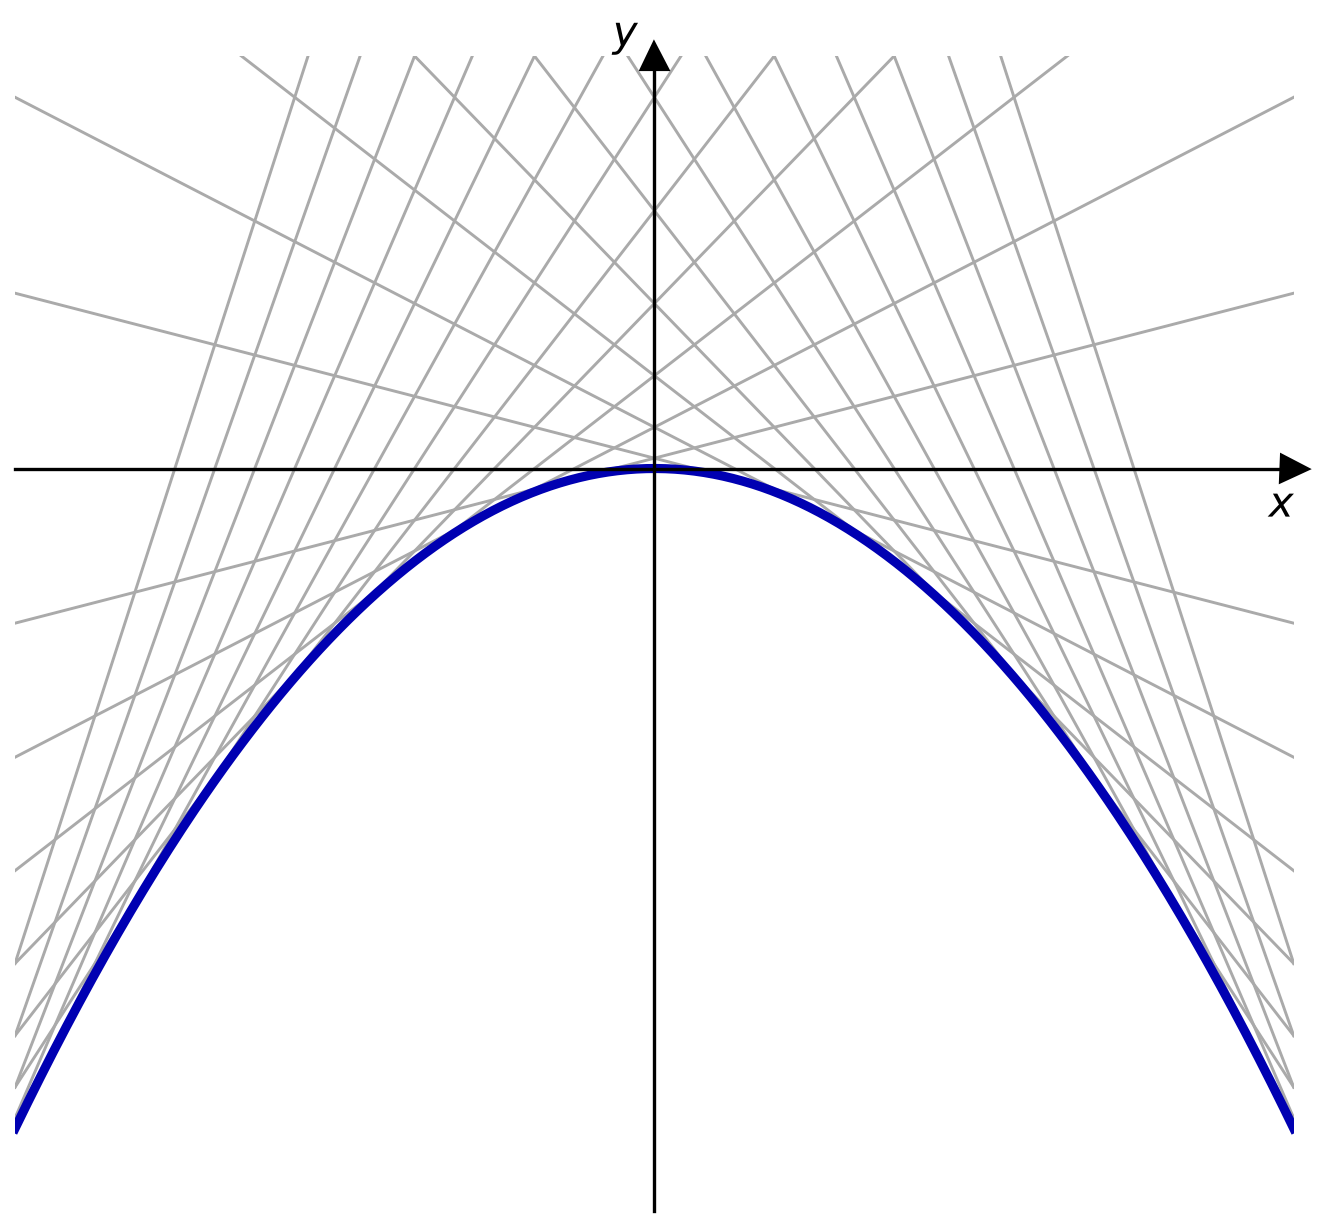
\includegraphics[width=0.5\linewidth]{pic/fig2.1_envelope.png}
    \caption{直线族 $y=cx+c^2$ 及其包络 $y=-\dfrac{x^2}{4}$}
\end{figure}

现在来看奇解. 令 $p=y'$，微分方程写为
\begin{equation}\label{equ:2.37}
F(x,y,p)=0.
\end{equation}

\begin{deff}
设 $y=\varphi(x)$ 是微分方程 (\ref{equ:2.37}) 的一个解. 若该解在每一点
$(x,\varphi(x))$ 处，都还有方程的另一个解经过这里，并与它在该点相切，
但该解的局部图像不与 $\varphi$ 重合，则称 $y=\varphi(x)$ 是方程的一个
\textbf{奇解}.
\end{deff}

从定义上看奇解和包络是十分类似的，事实上，他们之间确实有如下关系.

\begin{thm}\label{thm:2.5.2}
设 $y=\varphi(x)$ 是微分方程 (\ref{equ:2.37}) 的奇解，则它必是通解族
的包络. 反之，若通解族有包络，则该包络必是方程 (\ref{equ:2.37}) 的奇解.
\end{thm}
\begin{pf1}
$\Leftarrow$：设 $\Gamma: y=\varphi(x)$ 是通解族 $\Phi(x,y,C)=0$ 的包络，
则 $\Gamma$ 上每一点都有通解族中的一条曲线与 $\Gamma$ 在该点相切. 这说明
在该点处，$\Gamma$ 的切线斜率等于方程在该点的方向场方向，即
$F(x,\varphi(x),\varphi'(x))=0$，故 $\Gamma$ 是方程 (\ref{equ:2.37}) 的解.
又由包络定义，$\Gamma$ 不含通解族中任何曲线的非平凡弧段，特别地 $\Gamma$
本身不是通解族中的解，所以它是奇解.

$\Rightarrow$：设 $y=\varphi(x)$ 是奇解. 由奇解的定义，$\Gamma$ 上每一点
$(x,\varphi(x))$ 都有方程的另一解经过该点并与 $\Gamma$ 在该点相切；而方程除
奇解以外的解都包含在通解族中，故 $\Gamma$ 上每一点都有通解族中的曲线与之
相切. 另一方面，若 $\Gamma$ 含有通解族中某条曲线的非平凡弧段，则在这一段上
$\varphi$ 与通解族中的解重合，从而 $\varphi$ 本身属于通解族，与奇解的定义矛盾.
故按包络的定义，$\Gamma$ 是通解族的包络.
\end{pf1}

上面的定理揭示了奇解的几何本质，但使用它需要先求出通解族.
下面两个定理直接从方程本身出发给出奇解的判别方法.

\begin{thm}\label{thm:2.5.3}
设 $F(x,y,p)$ 在区域 $G\subset\R^3$ 内连续，且具有连续的一阶偏导数
$F_y,F_p$. 若 $y=\varphi(x)$（$x\in J$）是方程 (\ref{equ:2.37}) 的奇解，
并且 $(x,\varphi(x),\varphi'(x))\in G,\ x\in J$，则奇解 $y=\varphi(x)$
满足方程组
\begin{equation}\label{equ:2.38}
F(x,y,p)=0,\qquad F_p(x,y,p)=0,
\end{equation}
其中 $p=y'$.
\end{thm}
\begin{pf1}
设 $y=\varphi(x)$ 是奇解. 对 $\varphi$ 上每一点 $(x,\varphi(x))$，由奇解
定义，存在方程的另一个解 $\psi$ 在该点与 $\varphi$ 相切，即
\[
\varphi(x)=\psi(x),\qquad \varphi'(x)=\psi'(x)=p_0.
\]
于是点 $(x,\varphi(x),p_0)$ 同时是方程 (\ref{equ:2.37}) 关于 $\varphi$ 和
$\psi$ 的解. 这意味着从 $F(x,y,p)=0$ 中在 $(x,\varphi(x))$ 附近解不出唯一
的 $p$，因此由隐函数定理，函数 $F$ 在该点关于 $p$ 的偏导数必须为零，否则
由 $F_p\neq0$ 可唯一解出 $p=f(x,y)$，初值问题的解将唯一，不可能有两个
不同的解相切. 故 $F_p(x,\varphi(x),\varphi'(x))=0$，即奇解满足 (\ref{equ:2.38}).
\end{pf1}
\begin{rmk}
在定理 \ref{thm:2.5.3} 中，从方程组 (\ref{equ:2.38}) 中消去 $p$ 得到的曲线
称为 \textbf{p--判别曲线}.
\end{rmk}


\begin{thm}\label{thm:2.5.4}
设 $F(x,y,p)$ 在区域 $G\subset\R^3$ 内二阶连续可微，并且由 p--判别方程组
(\ref{equ:2.38}) 得到的函数 $y=\varphi(x)$（$x\in J$）是方程 (\ref{equ:2.37})
的解，且满足
\[
F_p(x,\varphi(x),\varphi'(x))\equiv0.
\]
若条件
\begin{equation}\label{equ:2.39}
F_y(x,\varphi(x),\varphi'(x))\neq0,\qquad
F_{pp}(x,\varphi(x),\varphi'(x))\neq0
\end{equation}
对一切 $x\in J$ 成立，则 $y=\varphi(x)$ 是方程 (\ref{equ:2.37}) 的奇解.
\end{thm}
\begin{pf1}
固定 $x_0\in J$，记 $y_0=\varphi(x_0)$，$p_0=\varphi'(x_0)$. 只需证明存在方程
(\ref{equ:2.37}) 的解 $\psi$，使
\[
\psi(x_0)=y_0,\qquad \psi'(x_0)=p_0,
\]
并且 $\psi$ 在 $x_0$ 的任何邻域内都不与 $\varphi$ 重合.

\textbf{第一步：将方程解出 $y$.} 由 $F_y(x_0,y_0,p_0)\neq0$ 及隐函数定理，
存在 $(x_0,p_0)$ 的邻域 $U$ 以及 $U$ 上的 $C^2$ 函数 $f(x,p)$，使得当 $y$
充分接近 $y_0$ 时
\[
F(x,y,p)=0\quad\Longleftrightarrow\quad y=f(x,p),\qquad (x,p)\in U,
\]
即 $F(x,f(x,p),p)\equiv0$. 因为 $\varphi$ 是方程 (\ref{equ:2.37}) 的解，所以
$(x,\varphi'(x))\in U$（$x$ 充分接近 $x_0$），且
\begin{equation}\label{equ:2.40}
\varphi(x)=f(x,\varphi'(x)).
\end{equation}
由隐函数求导公式
\[
f_x=-\frac{F_x}{F_y},\qquad f_p=-\frac{F_p}{F_y}.
\]
对 (\ref{equ:2.40}) 关于 $x$ 求导，并利用定理假设
$F_p(x,\varphi(x),\varphi'(x))\equiv0$ 与 $F_y\neq0$，得
\begin{equation}\label{equ:2.41}
\varphi'(x)=f_x(x,\varphi'(x)),\qquad
f_p(x,\varphi'(x))=0.
\end{equation}

\textbf{第二步：化为关于 $p$ 的方程.} 在 $U$ 内方程 (\ref{equ:2.37}) 与
$y=f(x,y')$ 等价. 记 $p=y'$，将其关于 $x$ 求导，得
\begin{equation}\label{equ:2.42}
p-f_x(x,p)=f_p(x,p)p'.
\end{equation}
记 $N(x,p)=p-f_x(x,p)$，$D(x,p)=f_p(x,p)$. 由 (\ref{equ:2.41})，$N$ 与 $D$
在曲线 $p=\varphi'(x)$ 上恒为零，故由中值积分公式可把它们写成
\[
N(x,p)=\bigl(p-\varphi'(x)\bigr)B(x,p),\qquad
D(x,p)=\bigl(p-\varphi'(x)\bigr)A(x,p),
\]
其中 $B,A$ 连续，且
\[
B(x_0,p_0)=N_p(x_0,p_0)=1-f_{xp}(x_0,p_0),\qquad
A(x_0,p_0)=D_p(x_0,p_0)=f_{pp}(x_0,p_0).
\]
对 $f_p=-F_p/F_y$ 关于 $p$ 求导，并利用
$F_p(x_0,y_0,p_0)=f_p(x_0,p_0)=0$，得
\[
f_{pp}(x_0,p_0)=-\frac{F_{pp}(x_0,y_0,p_0)}{F_y(x_0,y_0,p_0)}\neq0,
\]
故 $A(x_0,p_0)\neq0$；适当缩小 $U$，可设 $U$ 内 $A\neq0$. 于是当
$p\neq\varphi'(x)$ 时，方程 (\ref{equ:2.42}) 等价于
\begin{equation}\label{equ:2.43}
p'=\frac{B(x,p)}{A(x,p)}.
\end{equation}
右端在 $U$ 内连续，故由一阶方程解的存在性定理，存在 $x_0$ 的邻域 $I_0$
以及 $I_0$ 上的函数 $p(x)$，使 $p(x_0)=p_0$，并且 $p$ 在 $I_0$ 上满足
(\ref{equ:2.43}).

\textbf{第三步：$p(x)$ 与 $\varphi'(x)$ 只在 $x_0$ 处相交.} 由 (\ref{equ:2.43})，
\[
p'(x_0)=\frac{B(x_0,p_0)}{A(x_0,p_0)}
=\frac{1-f_{xp}(x_0,p_0)}{f_{pp}(x_0,p_0)}.
\]
另一方面，把恒等式 $F_p(x,\varphi(x),\varphi'(x))\equiv0$ 关于 $x$ 求导，得
\[
F_{px}+F_{py}p_0+F_{pp}\varphi''(x_0)=0,
\]
即
\[
\varphi''(x_0)
=-\frac{F_{px}(x_0,y_0,p_0)+p_0F_{py}(x_0,y_0,p_0)}
{F_{pp}(x_0,y_0,p_0)}.
\]
又由 $f_x=-F_x/F_y$、$f_p=0$ 及 $f_x(x_0,p_0)=p_0$（即 $F_x=-p_0F_y$）可得
\[
f_{xp}(x_0,p_0)
=-\frac{F_{xp}(x_0,y_0,p_0)+p_0F_{yp}(x_0,y_0,p_0)}{F_y(x_0,y_0,p_0)}.
\]
代入并利用 $f_{pp}=-F_{pp}/F_y$，得
\[
p'(x_0)-\varphi''(x_0)
=-\frac{F_y(x_0,y_0,p_0)}{F_{pp}(x_0,y_0,p_0)}\neq0.
\]
因此 $p(x)-\varphi'(x)$ 在 $x_0$ 处有单零点，即 $x_0$ 附近 $x\neq x_0$ 时
$p(x)\neq\varphi'(x)$.

\textbf{第四步：构造另一解，并验证它与 $\varphi$ 相切但不重合.} 令
\[
\psi(x)=f(x,p(x)),\qquad x\in I_0.
\]
则 $\psi(x_0)=f(x_0,p_0)=y_0$. 当 $x\neq x_0$ 时 $p(x)\neq\varphi'(x)$，
从而 $D(x,p(x))\neq0$，由 (\ref{equ:2.42})、(\ref{equ:2.43}) 得
\[
\psi'(x)=f_x(x,p(x))+f_p(x,p(x))p'(x)=f_x+(p-f_x)=p(x).
\]
再由 $\psi'$ 的连续性，$\psi'(x_0)=p(x_0)=p_0$. 故 $\psi$ 是方程
(\ref{equ:2.37}) 的解，且与 $\varphi$ 在 $x_0$ 处相切.

最后说明 $\psi$ 与 $\varphi$ 不局部重合. 由 (\ref{equ:2.41}) 中
$f_p(x,\varphi'(x))=0$，用带拉格朗日余项的二阶泰勒公式得
\[
\psi(x)-\varphi(x)=f(x,p(x))-f(x,\varphi'(x))
=\frac12 f_{pp}(x,\xi)\bigl(p(x)-\varphi'(x)\bigr)^2,
\]
其中 $\xi$ 介于 $p(x)$ 与 $\varphi'(x)$ 之间. 由 $f_{pp}(x_0,p_0)\neq0$ 及
$f_{pp}$ 的连续性，$x$ 充分接近 $x_0$ 时 $f_{pp}(x,\xi)\neq0$；又由第三步，
$x\neq x_0$ 时 $p(x)\neq\varphi'(x)$，故 $\psi(x)\neq\varphi(x)$.

由于 $x_0\in J$ 是任意的，$\varphi$ 上每一点都有方程 (\ref{equ:2.37}) 的另一个
解经过并与它在该点相切，且局部不重合. 按定义，$y=\varphi(x)$ 是奇解.
\end{pf1}


\begin{eg}
求方程 $y'^2-4y=0$ 的奇解.
\begin{pf2}
令 $F(x,y,p)=p^2-4y$，则方程组 (\ref{equ:2.38}) 为
\[
p^2-4y=0,\qquad 2p=0.
\]
由第二式得 $p=0$，代入第一式得 $y=0$. 故 p--判别曲线是 $y=0$.
将 $y=0$ 代入原方程，确实满足，因此它是方程的解. 下面验证充分条件
(\ref{equ:2.39}). 由于
\[
F_y=-4,\qquad F_{pp}=2,
\]
在 $y=0$ 上均不为零，故由定理 \ref{thm:2.5.4}，$y=0$ 是奇解.
易见原方程的通解为 $y=(x+C)^2$，而 $y=0$ 正是该抛物线族的包络.
\end{pf2}
\end{eg}


\section{近似解法}\label{sec:2.6}
\textbf{本节不是课程重点，准备考试的同学可以直接跳过.}


前面几节讨论的方程都能用初等函数或积分把解表示出来，但这样的方程只是极少数；
实际问题中给出的方程往往没有解析表达式，而是由函数或数据给出，根本无法用解析
方法求解. 因此有必要讨论方程的近似解法.

近似解法大体可以分为两类：
\begin{description}
\item[(i)] \textbf{解析近似法}：寻求解 $y=\varphi(x)$ 的近似解析表达式.
\item[(ii)] \textbf{数值解法}：计算解函数 $\varphi(x)$ 在一系列节点
\[
a=x_0<x_1<\cdots<x_n=b
\]
处的近似值 $y_i\approx\varphi(x_i)\ (i=1,\ldots,n)$. 相邻节点之间的距离
$h_i=x_{i+1}-x_i$ 称为\textbf{步长}；通常取等距节点，即 $h_i=(b-a)/n$.
\end{description}

本节总假设初值问题
\begin{equation}\label{equ:2.44}
\frac{dy}{dx}=f(x,y),\qquad y(x_0)=y_0
\end{equation}
在包含解曲线的区域内满足第 1 章定理 \ref{thm:1.1.2} 的条件，即 $f$ 连续且关于
$y$ 满足 Lipschitz 条件，从而其解存在且唯一. 为避免混淆，记初值问题 (\ref{equ:2.44})
的解为 $y=\varphi(x)$. 下面介绍四种常用的近似解法.

\subsection{逐次迭代法}
逐次迭代法源于第 1 章利用 Picard 迭代证明存在唯一性定理的方法，
设 $M=\max\limits_{R}|f(x,y)|$，$L$ 为 $f$ 关于 $y$ 的 Lipschitz 常数. 由第 1 章
的证明可知，初值问题 (\ref{equ:2.44}) 的解是 Picard 迭代序列
\begin{equation}\label{equ:2.45}
y_0(x)=y_0,\qquad
y_n(x)=y_0+\int_{x_0}^{x}f(t,y_{n-1}(t))\,dt,\quad n=1,2,\ldots
\end{equation}
的极限. 该序列在存在区间上一致收敛于解 $\varphi(x)$，因此迭代一定次数后，$y_n(x)$
就可以作为解的一个近似，迭代次数越多，近似程度越高.

下面给出误差估计. 由第 1 章的估计式 (\ref{equ:1.8})，
\[
|y_n(x)-y_{n-1}(x)|\le\frac{ML^{n-1}}{n!}|x-x_0|^n .
\]
于是
\begin{equation}\label{equ:2.46}
|\varphi(x)-y_n(x)|\le\sum_{k=n+1}^{\infty}|y_k(x)-y_{k-1}(x)|
\le\sum_{k=n+1}^{\infty}\frac{ML^{k-1}}{k!}|x-x_0|^k .
\end{equation}
记 $\lambda=L|x-x_0|$，则上式右端等于
\[
\frac{ML^n}{(n+1)!}|x-x_0|^{n+1}
\sum_{j=0}^{\infty}\frac{(n+1)!}{(n+1+j)!}\lambda^j .
\]
由于
\[
\frac{(n+1)!}{(n+1+j)!}
=\frac{1}{(n+2)(n+3)\cdots(n+1+j)}\le\frac{1}{2^j},
\]
故当 $\lambda\le1$ 时
\[
\sum_{j=0}^{\infty}\frac{(n+1)!}{(n+1+j)!}\lambda^j
\le\sum_{j=0}^{\infty}\left(\frac{\lambda}{2}\right)^j
=\frac{1}{1-\lambda/2}\le2 .
\]
因此
\begin{equation}\label{equ:2.47}
|\varphi(x)-y_n(x)|\le\frac{2ML^n}{(n+1)!}|x-x_0|^{n+1}.
\end{equation}

\begin{rmk}
误差估计 (\ref{equ:2.47}) 表明，$n$ 增大时误差按阶乘的速度趋于零. 但每一步迭代
都要计算一次积分，一般难以得到封闭形式；实际计算时通常需要借助数值积分，因此
该方法更多地用于理论分析.
\end{rmk}

\subsection{Taylor 级数法}
若解 $\varphi(x)$ 可以在 $x_0$ 处展开为幂级数，则可以用级数的前若干项来近似它：
\begin{equation}\label{equ:2.48}
\varphi(x)=\sum_{n=0}^{\infty}\frac{\varphi^{(n)}(x_0)}{n!}(x-x_0)^n,
\qquad |x-x_0|<\rho .
\end{equation}
这种求近似解的方法称为 \textbf{Taylor 级数法}. 它的理论基础是下面的定理.

\begin{thm}
设 $f(x,y)$ 在矩形区域
\[
R=\{(x,y):|x-x_0|\le a,\ |y-y_0|\le b\}
\]
上可以展开成 $(x-x_0)$ 与 $(y-y_0)$ 的幂级数，则初值问题 (\ref{equ:2.44}) 在
$x_0$ 的某邻域 $|x-x_0|<\rho$ 内存在唯一的解析解 $y=\varphi(x)$.
\end{thm}
\begin{pf1}
由定理 \ref{thm:1.1.2}，初值问题 (\ref{equ:2.44}) 在 $|x-x_0|\le h$ 上存在唯一解
$\varphi(x)$，故只需说明它解析. 考虑迭代序列 (\ref{equ:2.45}). $y_0$ 是常数，解析；
若 $y_{n-1}$ 解析，则 $f(x,y_{n-1}(x))$ 是解析函数的复合，仍然解析，再积分一次，
$y_n$ 也解析. 由第 1 章的估计式 (\ref{equ:1.8})，$\{y_n\}$ 在 $|x-x_0|\le h$ 上
一致收敛于 $\varphi$，从而在任意闭子区间上一致收敛. 一致收敛的解析函数列的极限仍解析
（Weierstrass 定理），故 $\varphi(x)$ 在 $|x-x_0|<\rho$ 内可展开为幂级数.
\end{pf1}

由上述定理，只需求出 $\varphi$ 在 $x_0$ 处的函数值及各阶导数，就能写出近似解. 由
方程本身 $\varphi'=f(x,\varphi(x))$ 依次求导，得
\begin{equation}\label{equ:2.49}
\frac{d^{j}\varphi}{dx^{j}}=\frac{d^{j-1}}{dx^{j-1}}f(x,\varphi(x))
=:f^{(j-1)}(x,\varphi(x))=\frac{d^{j-2}}{dx^{j-2}}(f_x+f_yf).
\end{equation}
把它们在 $x_0$ 处的值代入 (\ref{equ:2.48}) 并截断，即得
\begin{equation}\label{equ:2.50}
\varphi(x)\approx y_0+\sum_{j=1}^{N}\frac{f^{(j-1)}(x_0,y_0)}{j!}(x-x_0)^j,
\end{equation}
其中 $N$ 越大，近似程度越高.

\begin{rmk}
Taylor 级数法也可以作为逐步递推的公式使用. 设已算得 $y_n\approx\varphi(x_n)$，由
Taylor 公式
\begin{equation}\label{equ:2.51}
\varphi(x_{n+1})=\varphi(x_n)+h\varphi'(x_n)+\frac{h^2}{2!}\varphi''(x_n)
+\frac{h^3}{3!}\varphi'''(x_n)+\cdots,
\end{equation}
其中 $h=x_{n+1}-x_n$，各阶导数按 (\ref{equ:2.49}) 计算. 若只保留到 $h^p$ 项，
便得到 $p$ 阶的单步公式，局部截断误差为 $O(h^{p+1})$.
\end{rmk}

尽管 Taylor 公式在形式上很简单，但按 (\ref{equ:2.49}) 逐阶求导，运算量会随阶数
迅速增大，高阶导数几乎无法手工计算. 因此实际中通常不直接使用 Taylor 公式，而是
借鉴其"用更多阶的导数信息提高精度"的思想，构造只需要计算函数值的其它公式. 这
正是下面两种方法的出发点.

\subsection{Euler 折线法}
取等距节点 $x_n=x_0+nh$. 在 $x_n$ 处用向前差商代替导数：
\[
\frac{\varphi(x_{n+1})-\varphi(x_n)}{h}\approx\varphi'(x_n)=f(x_n,\varphi(x_n)).
\]
把 $\varphi(x_n)$ 换成已知的近似值 $y_n$，即得递推公式
\begin{equation}\label{equ:2.52}
y_{n+1}=y_n+hf(x_n,y_n),\qquad n=0,1,2,\ldots
\end{equation}
称为 \textbf{Euler 公式}.

从几何上看，Euler 公式就是在点 $(x_n,y_n)$ 处沿切线方向走一步，到达
$(x_{n+1},y_{n+1})$. 各步的线段首尾相接，得到一条折线，故 Euler 法也称为
\textbf{折线法}. 第一步的 $y_1$ 取自解曲线在初值点处的切线；由于 $y_1$ 一般
不等于 $\varphi(x_1)$，此后各步的切线就不再属于原解曲线，而是属于过当前近似点的
另一条解曲线，近似解逐步偏离真解.

\begin{figure}[htbp]
    \centering
    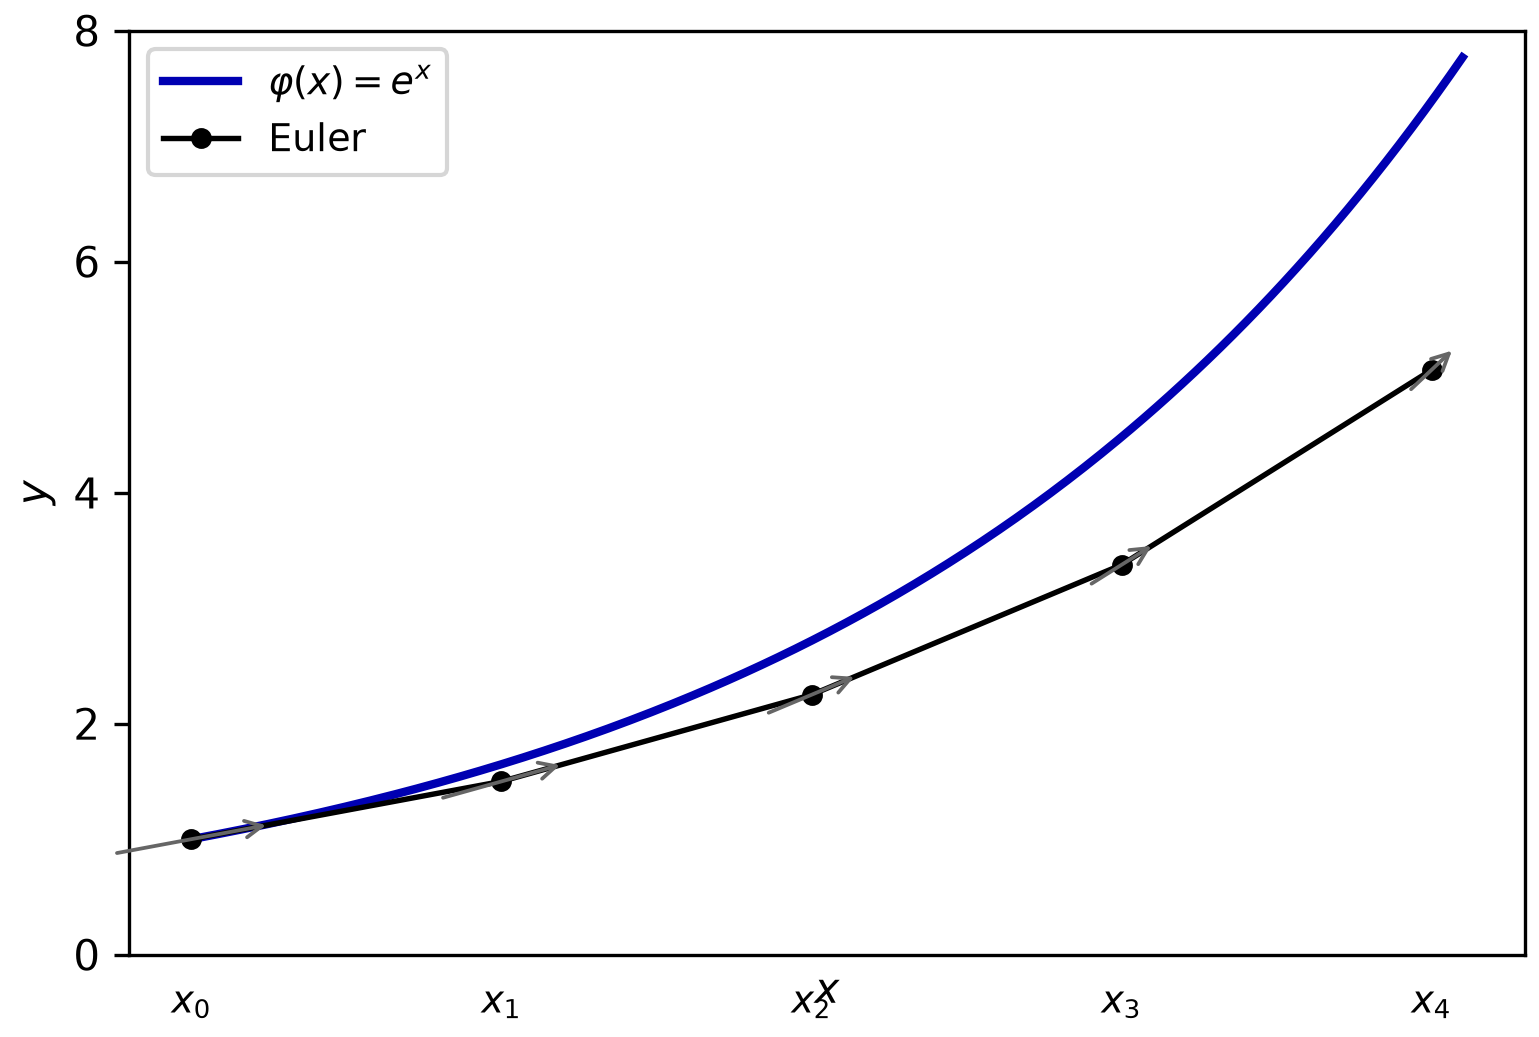
\includegraphics[width=0.6\linewidth]{pic/fig2.2_euler.png}
    \caption{Euler 折线法：方程 $y'=y,\ y(0)=1$ 取步长 $h=0.5$ 的折线与
    真解 $\varphi(x)=e^x$}
\end{figure}

下面估计误差. 设 $y_n=\varphi(x_n)$，即此前各步均无误差，则由 Taylor 公式
\[
\varphi(x_{n+1})-y_{n+1}
=\varphi(x_n)+h\varphi'(x_n)+\frac{h^2}{2}\varphi''(\xi_n)
-\left[\varphi(x_n)+hf(x_n,\varphi(x_n))\right]
=\frac{h^2}{2}\varphi''(\xi_n)=O(h^2),
\]
其中 $\xi_n\in(x_n,x_{n+1})$. 这是\textbf{局部截断误差}. 若在 $[x_0,x]$ 上共有
$N=(x-x_0)/h$ 步，则各步的局部误差累积起来，整体截断误差为 $O(h)$.

\begin{deff}
若某数值方法的局部截断误差为 $O(h^{p+1})$，则称它为 \textbf{$p$ 阶方法}，相应地
其整体截断误差为 $O(h^p)$.
\end{deff}
因此 Euler 法是一阶方法.

由此可见，对给定的节点，减小步长 $h$ 可以提高精度；而对固定的 $h$，误差随 $x$ 的
增大而迅速积累. 若要提高精度，或者进一步减小步长，或者只在初始点附近的较短区间
内进行计算.

为了提高精度，可以在每一步中多利用一些斜率信息. 一种办法是保留 Taylor 展开到
二阶：
\begin{equation}\label{equ:2.53}
y_{k+1}=y_k+hf(x_k,y_k)+\frac{h^2}{2}
\left[f_x(x_k,y_k)+f_y(x_k,y_k)f(x_k,y_k)\right],
\end{equation}
但这样需要计算 $f$ 的偏导数，使用起来并不方便. 改用如下做法：以 $x_n$ 与
$x_{n+1}$ 两点处斜率的算术平均值作为平均斜率，而 $x_{n+1}$ 处的斜率用已知的
$y_n$ 先预测出来：
\begin{equation}\label{equ:2.54}
\left\{
\begin{aligned}
K_1&=f(x_n,y_n),\\
K_2&=f(x_n+h,\,y_n+hK_1),\\
y_{n+1}&=y_n+\frac{h}{2}(K_1+K_2).
\end{aligned}
\right.
\end{equation}
其中 $\bar y_{n+1}=y_n+hK_1$ 是 $\varphi(x_{n+1})$ 的预测值，第三式是用梯形公式作校正.
公式 (\ref{equ:2.54}) 称为 \textbf{改进 Euler 法}，也称\textbf{预测--校正法}.

从几何上看，Euler 公式用的是区间左端点的斜率；若改用右端点的斜率，则得到
\begin{equation}\label{equ:2.55}
y_{n+1}=y_n+hf(x_{n+1},y_{n+1}),
\end{equation}
称为 \textbf{后退 Euler 公式}. 它是隐式公式，需要从 (\ref{equ:2.55}) 中解出
$y_{n+1}$，一般只能迭代求解. 梯形公式取两端点斜率的平均值
\[
y_{n+1}=y_n+\frac{h}{2}\left[f(x_n,y_n)+f(x_{n+1},y_{n+1})\right],
\]
它同样是隐式的；改进 Euler 公式 (\ref{equ:2.54}) 正是把其中的 $y_{n+1}$ 换成
预测值后所得的显式版本. 改进 Euler 法的局部截断误差为 $O(h^3)$，整体截断误差为
$O(h^2)$，是二阶方法.

在改进 Euler 公式中，平均斜率取的是等权的算术平均，第二个节点也固定取
$x_{n+1}$. 自然要问：权重是否必须相等？第二个节点是否必须取 $x_{n+1}$？把这两个
问题一般化，便得到下面的 Runge--Kutta 法.

\subsection{Runge--Kutta 法}
单步法的共同形式是
\[
y_{n+1}=y_n+h\Phi(x_n,y_n,h),
\]
即在点 $(x_n,y_n)$ 处取某一斜率 $\Phi$，沿直线走到 $(x_{n+1},y_{n+1})$. Euler 法
及其各种变形（如改进 Euler 法、后退 Euler 法）所能达到的最高精度只有二阶. 若要
进一步提高精度，就需要在每一步中提供更多、更精确的斜率信息.

由微分中值定理，存在 $\theta\in(0,1)$，使
\begin{equation}\label{equ:2.56}
\frac{\varphi(x_{n+1})-\varphi(x_n)}{h}=\varphi'(x_n+\theta h)
=f(x_n+\theta h,\,\varphi(x_n+\theta h))=k^*,
\end{equation}
于是
\[
\varphi(x_{n+1})=\varphi(x_n)+hk^*.
\]
$k^*$ 称为区间 $[x_n,x_{n+1}]$ 上的\textbf{平均斜率}. 只要对平均斜率给出一种近似
算法，就能导出一个相应的计算公式：
\begin{description}
\item[(i)] 取 $\theta=0$，$k^*\approx f(x_n,\varphi(x_n))=K_1$，即 Euler 公式；
\item[(ii)] 取 $\theta=1$，$k^*\approx f(x_{n+1},\varphi(x_{n+1}))=K_2$，即后退 Euler
公式；
\item[(iii)] 取 $k^*\approx(K_1+K_2)/2$，即梯形公式；
\item[(iv)] 取 $K_1=f(x_n,y_n)$，$K_2=f(x_n+h,y_n+hK_1)$，
$k^*=(K_1+K_2)/2$，即改进 Euler 公式.
\end{description}
可见上述方法都是对平均斜率 $k^*$ 的不同近似.

把改进 Euler 公式推广为
\begin{equation}\label{equ:2.57}
\left\{
\begin{aligned}
y_{i+1}&=y_i+h(\lambda_1K_1+\lambda_2K_2),\\
K_1&=f(x_i,y_i),\\
K_2&=f(x_i+ph,\,y_i+phK_1),
\end{aligned}
\right.
\end{equation}
其中 $\lambda_1,\lambda_2,p$ 为待定系数. 希望适当选取这些系数，使格式具有二阶精度，
即在 $y_i=\varphi(x_i)$ 的前提下，局部截断误差
\[
R_i=\varphi(x_{i+1})-y_{i+1}=O(h^3).
\]
为此把 $K_2$ 在 $(x_i,y_i)$ 处作 Taylor 展开：
\[
K_2=f(x_i,y_i)+phf_x(x_i,y_i)+phK_1f_y(x_i,y_i)+O(h^2)
=\varphi'(x_i)+ph\varphi''(x_i)+O(h^2),
\]
这里用了 $K_1=f(x_i,y_i)$ 以及 $\varphi''=f_x+f_yf$. 代入 (\ref{equ:2.57}) 得
\[
y_{i+1}=y_i+(\lambda_1+\lambda_2)h\varphi'(x_i)
+\lambda_2ph^2\varphi''(x_i)+O(h^3).
\]
而精确解在 $x_i$ 处的 Taylor 展开为
\[
\varphi(x_{i+1})=\varphi(x_i)+h\varphi'(x_i)+\frac{h^2}{2}\varphi''(x_i)+O(h^3).
\]
两式相减，要使 $R_i=O(h^3)$，只需
\begin{equation}\label{equ:2.58}
\lambda_1+\lambda_2=1,\qquad \lambda_2p=\frac{1}{2}.
\end{equation}
这是三个未知数、两个方程，因而有无穷多组解；所有满足 (\ref{equ:2.58}) 的格式统称为
\textbf{二阶 Runge--Kutta 格式}. 例如，取
\[
p=1,\qquad \lambda_1=\lambda_2=\frac{1}{2},
\]
就是改进 Euler 公式；而取
\[
p=\frac{1}{2},\qquad \lambda_1=0,\qquad \lambda_2=1,
\]
便得到
\[
y_{i+1}=y_i+hf\left(x_i+\frac{h}{2},\,y_i+\frac{h}{2}K_1\right),
\]
称为 \textbf{变形 Euler 公式}（中点公式）.

\begin{rmk}
二阶 Runge--Kutta 公式通过多计算一次函数值 $f$，避开了二阶 Taylor 公式所需的
$f$ 的导数. 在这个意义上，Runge--Kutta 方法可以看作 Taylor 级数法的变形.
\end{rmk}

上面的推导提示：若在 $[x_n,x_{n+1}]$ 上多预测几个点的斜率，再把它们的加权平均
作为平均斜率，就有可能构造出精度更高的公式，这就是 Runge--Kutta 方法的基本思想.
一般的 $m$ 级显式 Runge--Kutta 格式为
\begin{equation}\label{equ:2.59}
\left\{
\begin{aligned}
y_{n+1}&=y_n+h(\lambda_1K_1+\lambda_2K_2+\cdots+\lambda_mK_m),\\
K_1&=f(x_n,y_n),\\
K_2&=f(x_n+\alpha_2h,\,y_n+\beta_{21}hK_1),\\
K_3&=f(x_n+\alpha_3h,\,y_n+\beta_{31}hK_1+\beta_{32}hK_2),\\
&\ \vdots\\
K_m&=f(x_n+\alpha_mh,\,
y_n+\beta_{m1}hK_1+\cdots+\beta_{m,m-1}hK_{m-1}),
\end{aligned}
\right.
\end{equation}
其中 $\lambda_i\ (i=1,\ldots,m)$、$\alpha_i\ (i=2,\ldots,m)$ 与
$\beta_{ij}\ (i=2,\ldots,m;\ j=1,\ldots,i-1)$ 均为待定系数. 确定这些系数的步骤与
二阶情形完全相同：把各个 $K_i$ 在 $(x_n,y_n)$ 处展开，代入第一式后与精确解的
Taylor 展开逐项比较，使局部截断误差的阶尽可能高.

最常用的是四阶（经典）Runge--Kutta 格式：
\begin{equation}\label{equ:2.60}
\left\{
\begin{aligned}
y_n&=y_{n-1}+\frac{h}{6}(K_1+2K_2+2K_3+K_4),\\
K_1&=f(x_{n-1},y_{n-1}),\\
K_2&=f\left(x_{n-1}+\frac{h}{2},\,y_{n-1}+\frac{h}{2}K_1\right),\\
K_3&=f\left(x_{n-1}+\frac{h}{2},\,y_{n-1}+\frac{h}{2}K_2\right),\\
K_4&=f(x_{n-1}+h,\,y_{n-1}+hK_3).
\end{aligned}
\right.
\end{equation}
它具有四阶精度，即局部截断误差为 $O(h^5)$，整体截断误差为 $O(h^4)$.

\begin{rmk}
Runge--Kutta 法是单步法，计算 $y_{n+1}$ 只用到 $y_n$. 与 Taylor 级数法相比，它
不需要计算 $f$ 的偏导数，只需多次计算函数值，因而便于编程实现；但阶数越高，每步
所需的函数值计算次数越多，计算量也越大. 实际计算中，四阶 Runge--Kutta 法因精度
较高、使用方便而最为常见，步长 $h$ 则需在精度与计算量之间权衡选取.
\end{rmk}

至此介绍了四种近似解法. 逐次迭代法与 Taylor 级数法侧重于从解本身出发给出近似
表达式，Euler 法与 Runge--Kutta 法则给出了便于逐步计算的递推格式；后者精度更高，
也是实际计算中最常用的方法.


\section{一阶微分方程的应用}\label{sec:2.7}
由于一阶微分方程的应用不是本课程的重点，本节我们只介绍曲线族的等角轨线.
\subsection{曲线族的等角轨线}
\begin{deff}[(等角轨线)]
设给定单参数曲线族
\begin{equation}\label{equ:2.61}
\Phi(x,y,C)=0,
\end{equation}
其中 $C$ 为参数. 若一条曲线与族中的每一条曲线都相交，且交点处的交角恒等于定角
$\theta\ (0<\theta\le\pi/2)$，则称这条曲线为曲线族 (\ref{equ:2.61}) 的
\textbf{等角轨线}；当 $\theta=\pi/2$ 时，等角轨线称为\textbf{正交轨线}.
\end{deff}

求等角轨线的关键在于找出曲线族所满足的微分方程. 从 (\ref{equ:2.61}) 及其对
$x$ 求导所得的式子
\[
\Phi_x(x,y,C)+\Phi_y(x,y,C)y'=0
\]
中消去参数 $C$，便得到曲线族的微分方程
\begin{equation}\label{equ:2.62}
\frac{dy}{dx}=f(x,y).
\end{equation}
于是问题转化为：已知族中曲线的斜率 $f(x,y)$，求与之交成定角的曲线的斜率.

\begin{thm}\label{thm:2.7.1}
设曲线族 (\ref{equ:2.61}) 所满足的微分方程为 (\ref{equ:2.62})，则与族中曲线
交角为 $\theta\ (0<\theta<\pi/2)$ 的等角轨线满足
\begin{equation}\label{equ:2.63}
\frac{dy}{dx}=\frac{f(x,y)+\tan\theta}{1-f(x,y)\tan\theta}
\end{equation}
或
\begin{equation}\label{equ:2.64}
\frac{dy}{dx}=\frac{f(x,y)-\tan\theta}{1+f(x,y)\tan\theta},
\end{equation}
特别地，正交轨线满足
\begin{equation}\label{equ:2.65}
\frac{dy}{dx}=-\frac{1}{f(x,y)}.
\end{equation}
\end{thm}
\begin{pf1}
设族中曲线在点 $(x,y)$ 处切线的倾斜角为 $\alpha$，则 $\tan\alpha=f(x,y)$. 等角
轨线与它的交角为 $\theta$，故轨线切线的倾斜角为 $\alpha+\theta$ 或 $\alpha-\theta$.
对两者分别用正切和角公式，即得 (\ref{equ:2.63}) 与 (\ref{equ:2.64})，它们给出位于
族曲线两侧的两族轨线.

当 $\theta=\pi/2$ 时，$\tan\theta$ 不存在，上述公式失效. 但此时两切线垂直，斜率
互为负倒数，即得 (\ref{equ:2.65}). 若在交点处 $f(x,y)=0$，则正交轨线在该点的切线
竖直，应写成 $x=$ 常数. 
\end{pf1}

\begin{eg}
求圆族 $x^2+y^2=C^2\ (C>0)$ 的正交轨线.
\begin{pf2}
对 $x^2+y^2=C^2$ 求导得 $2x+2yy'=0$，即 $y'=-\dfrac{x}{y}$. 由 (\ref{equ:2.65})，
正交轨线满足
\[
\frac{dy}{dx}=\frac{y}{x},
\]
分离变量并积分得 $\ln|y|=\ln|x|+C_1$，即 $y=C_2x$. 这是一族过原点的直线.
另外，$x=0$（即 $y$ 轴）也是正交轨线.
\end{pf2}
\end{eg}

\begin{figure}[H]
    \centering
    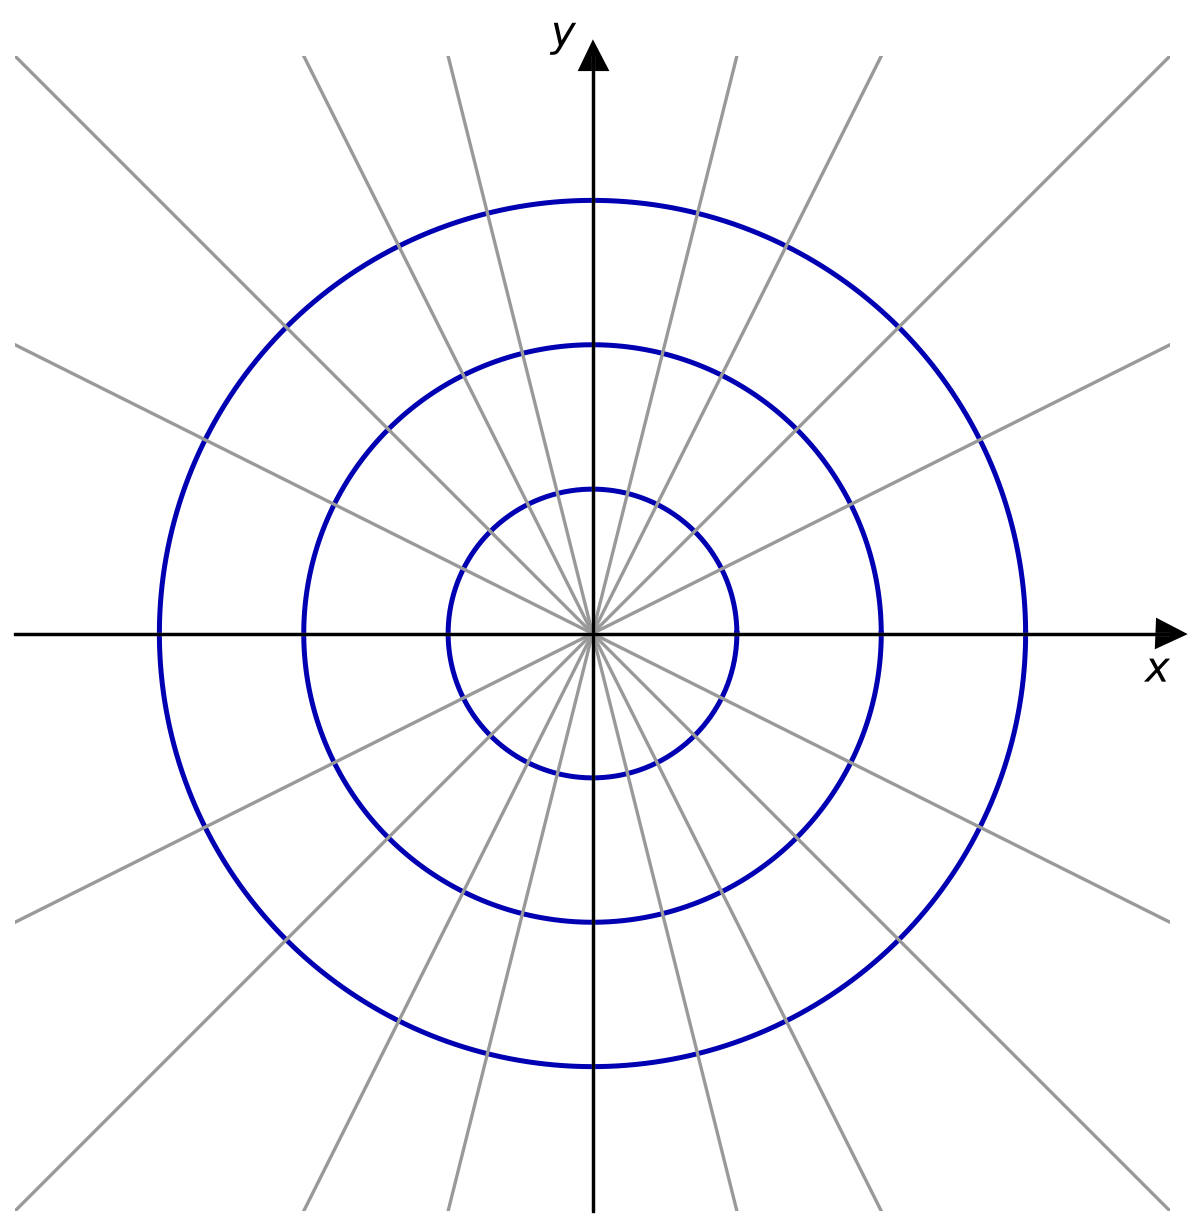
\includegraphics[width=0.45\linewidth]{pic/fig2.3_orthogonal.png}
    \caption{圆族 $x^2+y^2=C^2$（蓝）与其正交轨线 $y=C_2x$ 及 $x=0$（灰）}
\end{figure}
